\chapter{The Compact Muon Solenoid experiment}
\label{The Compact Muon Solenoid experiment}
The Compact Muon Solenoid (CMS) experiment is one of the main particle detectors
at the LHC currently in use at CERN, along with ATLAS, ALICE, and LHCb.

It is a general purpose detector, i.e., it is designed to observe all particle
interactions in a collision.
CMS is also designed to be a hermetic detector, i.e., it attempts to let no known particles
escape the detector undetected.
This is because the decay of particles can produce new, neutral, particles that do not interact with
any part of the detector.
With the hermetic design, imbalance in momentum and energy can be detected, and
the production of these non-interacting particles can be inferred.

The current goals of the CMS detector are to provide precise measurements of the
properties of the recently discovered Higgs boson, as well as to search for new
physics (also referred to as physics beyond the Standard Model) and thereby
answer currently open questions in particle physics. What are the properties of
QCD (Quantum ChromoDynamics) in extreme conditions? What are the differences
between matter and antimatter particles?
% TODO more of these

% The purpose of the CMS detector is to search for new physics phenomena (also
% referred to as physics beyond the Standard Model) such as Supersymmetry, and to
% provide precise measurements of the properties of the recently discovered Higgs boson.

It was credited with the discovery of the Higgs boson in 2012, together with the
ATLAS (A Toroidal LHC ApparatuS) detector.
One of the events displaying a candidate Higgs decay into two electrons and two
muons is displayed in figure \ref{fig:higgs}.

% \begin{figure}
%   \centering
%   \includegraphics[width=\textwidth]{images/higgs}
%   \caption{Observed candidate decay of Higgs$ \rightarrow ZZ^\ast (ee\mu\mu)$,
%   where the green and red lines emanating from the center are two electrons and
%   two muons, respectively.\cite{higgs}}
%   \label{fig:higgs}
% \end{figure}

\begin{figure}
  \centering
  \begin{minipage}[t]{0.49\textwidth}
    \includegraphics[width=\textwidth]{images/higgs}
    \caption{Observed candidate decay of Higgs$ \rightarrow ZZ^\ast (ee\mu\mu)$,
    where the green and red lines emanating from the center are two electrons and
    two muons, respectively.\cite{higgs}}
    \label{fig:higgs}
  \end{minipage}
  \hfill
  \begin{minipage}[t]{0.49\textwidth}
    \includegraphics[width=\textwidth]{images/higgs2}
    \caption{Observed candidate decay of  Higgs$ \rightarrow \gamma\gamma$, the
    green lines eminating from the center are two photons.\cite{higgs2}}
    \label{fig:higgs2}
  \end{minipage}
\end{figure}

CMS is designed to be capable to observe particles resulting from proton-proton
collisions with a center-of-mass energy of $\sqrt{s} = 14$TeV produced by the
Large Hadron Collider (LHC).
Currently the LHC provides collisions with a center-of-mass energy of
$\sqrt{s} = 13$TeV.

More information about the LHC experiments can be found in the book
`The CERN Large Hadron Collider: Accelerator and Experiments`\cite{CMS_Experiment}.

\section{The structure of CMS}
\subsection{Silicon Tracker}
The tracker can reconstruct the path of passing muons, electrons, and charged
hadrons. Because it is closest to the collisions, the decays of very short-lived particles (e.g.
beauty quarks)\cite{aboutCMS} can be detected.

It makes very precise measurements on the location of particles (with an accuracy
up to \SI{10}{\micro\meter}). Accompanied by a magnetic field, the momentum of
these particles can be determined.
Yet this section tries to be as unobstructive to particles as possible. This is
accomplished by using a silicon microstrip design, minimizing the volume of material that
can obstruct particles.

Being the closest to the proton-proton collisions, this part of the detector is
the one that has to endure the most radiation.
\subsection{Electromagnetic Calorimeter}
The Electromagnetic Calorimeter (ECAL) is a set of 75.848 lead tungstate (\ce{PbWO4}) crystals
with a total weight of about 100 tonnes.

It is designed to stop and measure the energy of passing electrons and photons.

These crystals produce light in the form of electromagnetic photon showers (see image \ref{fig:cms_slice})
that are measured by photodetectors (either avalanche photodiodes or vacuum phototriodes).

These crystals are very radiation hard and can reverse their radiation damage when
kept in room temperature (during beam time they are cooled to 0.1\degree C).
\subsection{Hadronic Calorimeter}
The Hadronic Calorimeter (HCAL) is designed to detect hadrons (i.e. particles
produced of quarks) and gluons.

This part of the detector is organized in several layers of dense absorbing materials and scintillators,
a combination of steel and plastic, where the plastic produces a light pulse when a particle flows through it.

The fact that the HCAL is housed inside the solenoid is one of the biggest
differences between the ATLAS and the CMS experiment.
\subsection{Superconducting Solenoid}
The design of CMS had a high focus on achieving the highest possible magnetic
field. To achieve this CMS has been equipped with one large superconducting
solenoid, capable of generating a magnetic field of \SI{4}{\tesla}.

This allows for very precise momentum readings by analyzing the arcs of charged
particles. It also provides sufficient return flux outside
the solenoid to be used by the muon chambers (about \SI{2}{\tesla}).
\subsection{Muon Chambers}
Muons (and neutrinos) are the only particles that can pass the previously
mentioned sections without losing most (if not all) of their energy.

The loss of energy as a particle travels through matter is  described by the
Bethe equation (\ref{eq:bethe}). Because of the characteristics of Muons,
this equation states that muons will not
release much of their energy as they pass through material.

Combined with the fact that these particles have high mass, this makes them very difficult to stop.

\begin{equation} \label{eq:bethe}
- \left\langle\frac{dE}{dx}\right\rangle = \frac{4 \pi}{m_e c^2} \cdot \frac{nz^2}{\beta^2} \cdot \left(\frac{e^2}{4\pi\varepsilon_0}\right)^2 \cdot \left[\ln \left(\frac{2m_e c^2 \beta^2}{I \cdot (1-\beta^2)}\right) - \beta^2\right]
\end{equation}

% $- \left\langle\frac{dE}{dx}\right\rangle = \frac{4 \pi}{m_e c^2} \cdot \frac{nz^2}{\beta^2} \cdot \left(\frac{e^2}{4\pi\varepsilon_0}\right)^2 \cdot \left[\ln \left(\frac{2m_e c^2 \beta^2}{I \cdot (1-\beta^2)}\right) - \beta^2\right]$


Since muons can't be easily stopped, the muon chambers rely
instead on the strong magnetic field to measure the curvature of these charged
particles, and thereby measuring their energy.
The muon chambers are composed of three components, the Resistive Plate Chambers
(RPC), Drift Tubes (DT), and Cathode Strip Chambers (CSC).


\begin{figure}
  \centering
  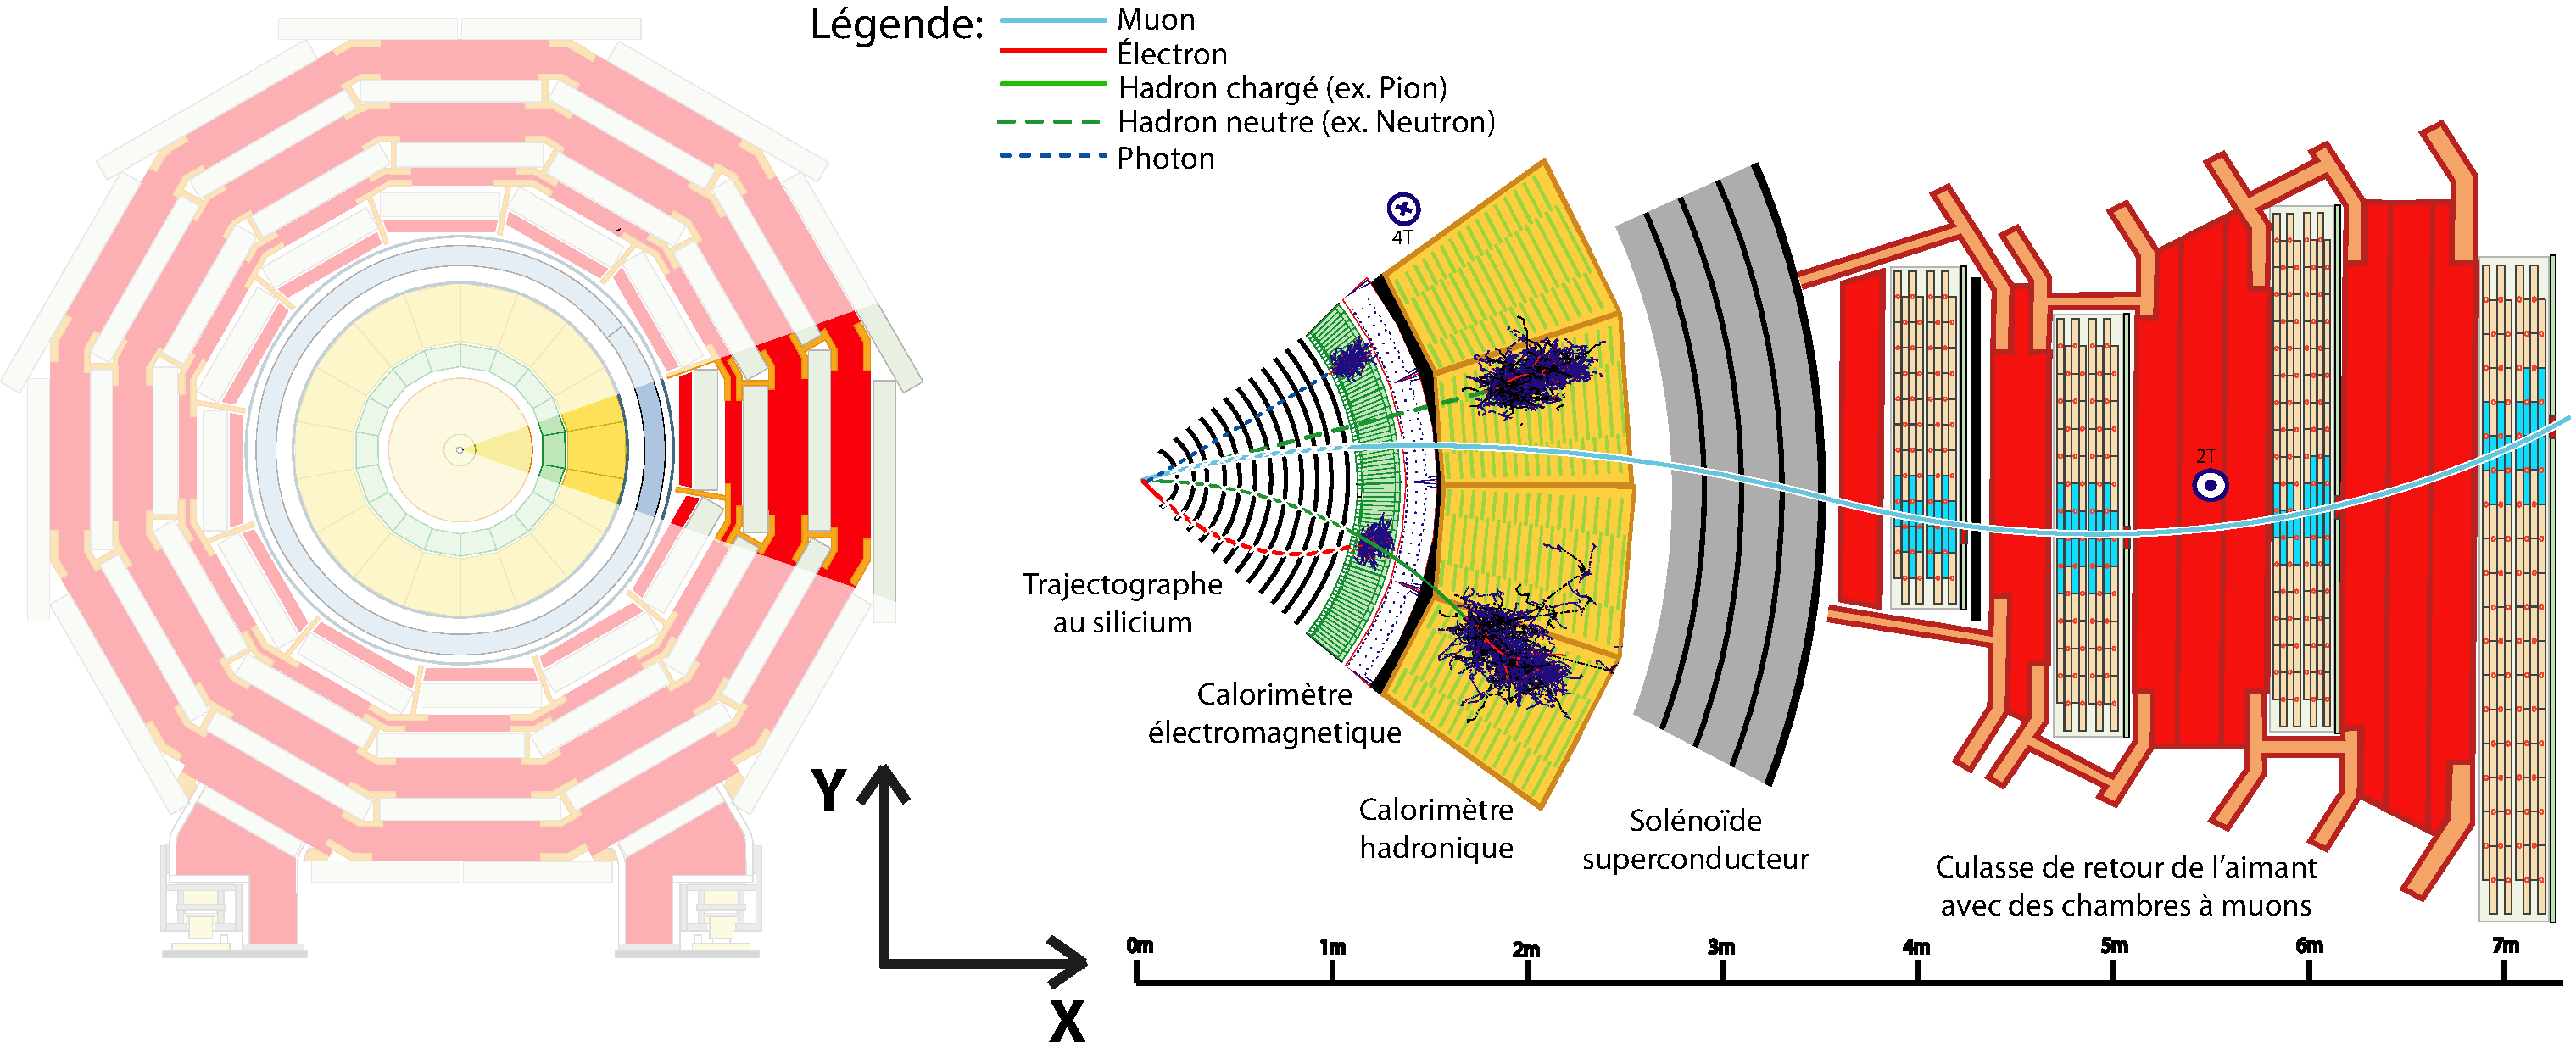
\includegraphics[width=\textwidth]{images/cms_slice}
  \caption{A transversal slice through the CMS detector, demonstrating the various
  sections of the detector and their designed functions.\cite{cms_slice}}
  \label{fig:cms_slice}
\end{figure}





% \section{The Level-1 Trigger}
% LHC produces proton-proton collisions in the center of the CMS detector. This is
% accomplished by providing a periodic moment bunch crossing in the detector.
% The LHC is currently designed to provide periodic bunch crossing in the detector
% at a rate of 40MHz and with a centre-of-mass energy of $\sqrt{s} = 14$TeV.
%
% The current luminosity of the beam in LHC will result in an average of ~40-50
% proton-proton collisions per bunch crossing, resulting in around 2MB of data
% generated by the sensor electronics.
%
% At a rate of 40MHz this will effectively produce a data stream of 80TB/s.
% This is too much for any storage system to handle, so a system is needed to
% filter this data so only data that looks interesting is retained.
%
% To handle this huge data stream, the level-1 (L1) trigger system is developed.
% Its purpose is to reduce the data stream to a maximum of 200 GB/s by filtering
% the collision rate to 100kHz.
% This reduction of data is done real-time and is programmed into field-programmable
% gate arrays (FPGAs) inside the detector.
%
% The bunch crossing frequency of 40MHz implies the L1 trigger has very little time
% to fully analyze a bunch crossing and decide which collisions to keep for further
% analysis.
%
% Currently, the time it takes for the L1 trigger to make a decision is \SI{3.2}{\micro\second},
% the time it takes for 128 bunch crossings to pass.
% Therefore all sensors have a buffer that can contain all the data of 128 bunch
% crossings. When the L1 trigger issues a L1 ACCEPT directive, the buffers are
% read and stored.
%
% This data is then passed to the high level trigger (HLT), to be further reduced
% to a 10 Hz collision rate.
% The high level trigger is also called the offline software because, unlike the
% L1 trigger, the calculations are not performed real-time.
% More information about the HLT can be found in the Phase II technical proposal
% \cite{TS_Phase2}.
